\documentclass[hyperref={pdftex,pdfpagemode=none,pdfstartview=FitH},10pt]{beamer}
\usepackage[english]{babel}
\usepackage{times}
%\usepackage{mathptmx,helvet}
\usepackage{amsmath,amssymb}
\usepackage{subfigure,graphicx,tabularx,booktabs,colortbl}
\usepackage{amssymb,amsmath,amsthm,times,graphicx,subfigure,tabularx,booktabs,colortbl,multirow,threeparttable,graphics}
\usepackage{movie15}

\usepackage{color}
\newcommand{\hilight}[1]{\colorbox{green}{#1}}

\newcommand{\norm}[1]{\ensuremath{\left\| #1 \right\|}}
\newcommand{\bracket}[1]{\ensuremath{\left[ #1 \right]}}
\newcommand{\braces}[1]{\ensuremath{\left\{ #1 \right\}}}
\newcommand{\parenth}[1]{\ensuremath{\left( #1 \right)}}
\newcommand{\refeqn}[1]{(\ref{eqn:#1})}
\newcommand{\reffig}[1]{Fig. \ref{fig:#1}}
\newcommand{\tr}[1]{\mbox{tr}\ensuremath{\negthickspace\bracket{#1}}}
\newcommand{\trs}[1]{\mbox{tr}\ensuremath{\bracket{#1}}}
\newcommand{\deriv}[2]{\ensuremath{\frac{\partial #1}{\partial #2}}}
\newcommand{\T}{\ensuremath{\mathsf{T}}}
\newcommand{\SO}{\ensuremath{\mathsf{SO}(3)}}
\newcommand{\G}{\ensuremath{\mathsf{G}}}
\renewcommand{\d}{\ensuremath{\mathfrak{d}}}
\newcommand{\so}{\ensuremath{\mathfrak{so}(3)}}
\renewcommand{\Re}{\ensuremath{\mathbb{R}}}
\newcommand{\aSE}[2]{\ensuremath{\begin{bmatrix}#1&#2\\0&1\end{bmatrix}}}
\newcommand{\SE}{\ensuremath{\mathrm{SE(3)}}}
\newcommand{\se}{\ensuremath{\mathfrak{se}(3)}}
\renewcommand{\S}{\ensuremath{\mathbb{S}}}
\newcommand{\abs}{\mathop{\mathrm{abs}}\nolimits}


\renewcommand{\r}{\mathbf{r}}
\renewcommand{\u}{\mathbf{u}}
\newcommand{\y}{\mathbf{y}}
\newcommand{\x}{\mathbf{x}}

\definecolor{RoyalBlue}{rgb}{0.25,0.41,0.88}
\def\Emph{\textcolor{RoyalBlue}}

\definecolor{mygray}{gray}{0.9}
\definecolor{tmp}{rgb}{0.804,0.941,1.0}
\setbeamercolor{numerical}{fg=black,bg=tmp}
\setbeamercolor{exact}{fg=black,bg=red}

\mode<presentation> {
  \usetheme{Warsaw}
  \usefonttheme{serif}
  \setbeamercovered{transparent}
}

\setbeamertemplate{footline}%{split theme}
{%
  \leavevmode%
  \hbox{\begin{beamercolorbox}[wd=.5\paperwidth,ht=2.5ex,dp=1.125ex,leftskip=.3cm,rightskip=.3cm plus1fill]{author in head/foot}%
    \usebeamerfont{author in head/foot}\insertshorttitle
  \end{beamercolorbox}%
  \begin{beamercolorbox}[wd=.5\paperwidth,ht=2.5ex,dp=1.125ex,leftskip=.3cm plus1fill,rightskip=.3cm]{title in head/foot}%
    \usebeamerfont{title in
    head/foot}\insertframenumber/\inserttotalframenumber
  \end{beamercolorbox}}%
  \vskip0pt%
} \setbeamercolor{box}{fg=black,bg=yellow}

\title[Nonlinear Observability Measure for Relative Orbit Determination]
{Nonlinear Observability Measure for Relative Orbit
\\
Determination with Angles-Only Measurements}

\author{
Evan Kaufman\\
{\footnotesize\selectfont Department of Mechanical and Aerospace Engineering,\\
The George Washington University, Washington DC}
$ $\\
\vspace*{0.015\columnwidth}
T. Alan Lovell\\
{\footnotesize\selectfont Air Force Research Laboratory,\\ Kirtland AFB, Albuquerque NM}
$ $\\
\vspace*{0.015\columnwidth}
Taeyoung Lee\\
{\footnotesize\selectfont Department of Mechanical and Aerospace Engineering,\\
The George Washington University, Washington DC}
}


%\institute[GWU]{\footnotesize\selectfont
%$^*$ Air Force Research Laboratory, Kirtland AFB, Albuquerque NM\\$ $\\
%Department of Mechanical and Aerospace Engineering\\
%George Washington University, Washington DC\\$ $\\}

\date{\vspace*{-0.8cm}\\AAS/AIAA Spaceflight Mechanics Meeting 2015\vspace*{0.1cm}\\
\footnotesize\selectfont (Supported by AFRL Summer Faculty and Space Scholars Programs,\\ NSF Grants CMMI-\#1029551, \#1335008, and CNS-\#1337722)}

%	\graphicspath{{/Users/tylee@seas.gwu.edu/Documents/Seminar/ISSFD14/Figs/}}
%\graphicspath{{/Users/evankaufman/Google Drive/FDCL/Evan/Publications/AAS 2015 OD EKF/Presentation/Figs}}
\graphicspath{{Figs/}}



\begin{document}

\begin{frame}
  \titlepage
\end{frame}


\section*{}
\subsection*{I. Introduction}


\begin{frame}
\frametitle{Introduction}
\begin{itemize}
\item Space Relative Navigation
	\begin{itemize}
	\item Space-based orbit determination
	\item Determine relative orbital properties between satellites by on-board measurements
	\item Critical for accurate formation control and close-proximity missions\\
	\end{itemize}
\end{itemize}

\vfill
\centerline{
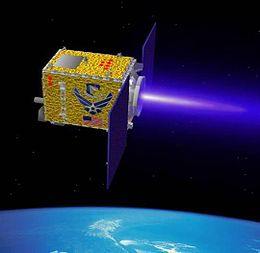
\includegraphics[height=2.7cm]{XSS11.jpg}\hspace*{0.2cm}
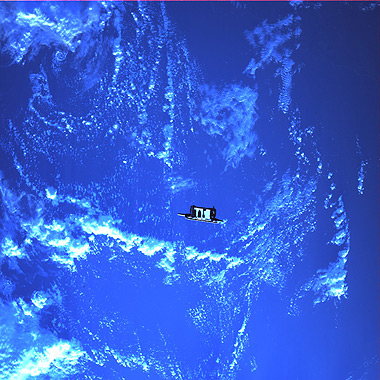
\includegraphics[height=2.7cm]{DLRPrisma.jpg}\hspace*{0.2cm}
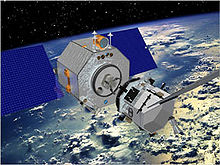
\includegraphics[height=2.7cm]{OrbitalExpress.jpg}}
\centerline{\scriptsize\selectfont
AFRL XSS-11\hspace*{1.5cm} DLR PRISMA\hspace*{1.5cm} DARPA Orbital Express}
\end{frame}


\begin{frame}
\frametitle{Introduction}

\begin{itemize}
\item Space-Based Space Surveillance (SBSS)
	\begin{itemize}
	\item Detection, collection, identification and tracking of man-made space objects from deep space to low-earth orbits
%	\item Ground-based optical systems are limited to clear weather, night-time observations
	\item SBSS provides all-weather, day and night, near real-time space situation awareness data
	\item Ability to search for lost/unknown space objects in deep space
	\end{itemize}
	\vspace*{0.3cm}\pause
\item Relative Orbit Determination with \Emph{Angles-Only Measurements}
	\begin{itemize}
	\item Lines-of-sight between satellites are measured by optical sensors
	\item Optical sensors have desirable properties of being low-cost and minimal maintenance
	\item Range is not available:\\ \Emph{Unobservable for linearized relative orbital dynamics} [Woffinden 09]
	\item Observability for nonlinear relative orbital dynamics has been unknown
	\end{itemize}
\end{itemize}

\vspace*{0.3cm}\pause
    \centerline{
    \begin{beamercolorbox}[wd=10.68cm,sep=0.2cm,center,shade=on]{numerical}
        \small\bfseries\selectfont Goal: Investigative Observability for \textit{Nonlinear} Relative Orbital Dynamics
    \end{beamercolorbox}}

\end{frame}

\section*{}
\subsection*{II. Problem Formulation}


\begin{frame}
\frametitle{Relative Orbit Dynamics}

\begin{columns}
\begin{column}{6.5cm}
\footnotesize\selectfont
\only<1>{
\setlength{\unitlength}{1cm}
\begin{picture}(7,7)(0,0)
\put(0,0){\includegraphics[width=7cm]{PF0.pdf}}
\put(3.2,1.3){$a$}
\put(4.8,2.8){Chief}
\end{picture}
}
\only<2>{
\setlength{\unitlength}{1cm}
\begin{picture}(7,7)(0,0)
\put(0,0){\includegraphics[width=7cm]{PF1.pdf}}
\put(3.2,1.3){$a$}
\put(6.15,3.55){$x$}
\put(4.5,4.5){$y$}
\put(4.8,2.8){Chief}
\end{picture}
}
\only<3>{
\setlength{\unitlength}{1cm}
\begin{picture}(7,7)(0,0)
\put(0,0){\includegraphics[width=7cm]{PF2.pdf}}
\put(3.2,1.3){$a$}
\put(6.15,3.55){$x$}
\put(4.5,4.5){$y$}
\put(5.7,4.3){$\mathbf{r}$}
\put(4.8,2.8){Chief}
\put(5.3,6.1){Deputy}
\end{picture}
}
\end{column}
%
\begin{column}{6cm}
\begin{itemize}
\item Chief Satellite
	\begin{itemize}
	\item On a circular orbit
	\item Orbital radius $a$ is known
	\end{itemize}
\vspace*{0.3cm}\pause
\item Local-vertical, local-horizontal (LVLH) frame
	\begin{itemize}
	\item $x$--axis: radial
	\item $y$--axis: tangent to the path
	\item $z$--axis: normal to the orbital plane
	\item Rotating about the $z$--axis with $\mathbf{\omega}=\sqrt{\frac{\mu}{a^3}}$.
	\end{itemize}
\vspace*{0.3cm}\pause
\item Deputy Satellite
	\begin{itemize}
	\item On an unknown, arbitrary orbit\\
	\item Relative position $\mathbf{r}\in\Re^3$

	\end{itemize}
\end{itemize}
\end{column}
\end{columns}
\end{frame}


\begin{frame}
\frametitle{Relative Orbit Dynamics}

\begin{itemize}
\item Nonlinear Equations of Motion (Two-Body Gravity Only)
	\begin{itemize}
	\item State vector: $\mathbf{x}=[\r,\;\dot\r]\in\Re^6$
	\item State equation: $\dot \x = f(\x)$, where
\begin{align*}
f(\mathbf{x}) 
=\begin{bmatrix}
\dot \r \\
-2\omega\times \dot\r - \omega\times(\omega\times \r_a) -\dfrac{\mu \r_a}{\|\r_a\|^3}
\end{bmatrix}.
\end{align*}
($\r_a=\r+[a,0,0]^T$: position vector of deputy from the center of Earth)
	\end{itemize}
\vspace*{0.3cm}\pause
\item Hill-Clohessey-Wiltshire (HCW) Equations
	\begin{itemize}
	\item Linearization of above ODEs about $\x=0$: $\delta\dot\x = A\delta \x$, where
\begin{align*}
A=\deriv{f(\x)}{\x}\bigg|_{\x=0}
=\begin{bmatrix}
0 & 0 & 0 & 1 & 0 & 0\\
0 & 0 & 0 & 0 & 1 & 0\\
0 & 0 & 0 & 0 & 0 & 1\\
3n^2 & 0 & 0 & 0 & 2n & 0\\
0 & 0 & 0 & -2n & 0 & 0\\
0 & 0 & -n^2 & 0 & 0 & 0
\end{bmatrix}.
\end{align*}
	\end{itemize}
\end{itemize}
\end{frame}



\begin{frame}
\frametitle{Line-of-sight Measurements}

\begin{columns}
\begin{column}{6.5cm}
\footnotesize\selectfont
\setlength{\unitlength}{1cm}
\begin{picture}(7,7)(0,0)
\put(0,0){\includegraphics[width=7cm]{PF3.pdf}}
\put(3.2,1.3){$a$}
\put(6.15,3.55){$x$}
\put(4.5,4.5){$y$}
\put(5.6,4.0){$\y$}
\put(4.8,2.8){Chief}
\put(5.3,6.1){Deputy}
\end{picture}
\end{column}
%
\begin{column}{6cm}
\begin{itemize}
\item Measurements
	\begin{itemize}
	\item Line-of-sight from chief to deputy is measured
	\item Measurement:
	\begin{align*}
	\y = \frac{\r}{\|\r\|}\in\Re^3
	\end{align*}
	(unit-length: $\|\y\|$=1)
	\end{itemize}
\vspace*{0.3cm}\pause
\item Relative Orbit Determination
	\begin{itemize}
	\item Wish to determine the relative orbit $\x=[\r,\dot\r]$ completely from $\y(t)$ only
	\end{itemize}	
\end{itemize}	
\end{column}
\end{columns}
\end{frame}

\section*{}
\subsection*{III. Observability}


\begin{frame}
\frametitle{Observability of HCW Equations}

\begin{itemize}
\item Solution of the Linear HCW Equation
	\begin{itemize}
	\item Let $\x(t)$ be the solution with an initial condition $\x(t_0)=\x_0$.
	\begin{align*}
	\x(t) = \exp(A(t-t_0)) \x_0
	\end{align*}
	\item \Emph{Homogeneity property}: let $\x'(t)$ be the solution with a \textit{scaled} initial condition $\x'(t_0)=\alpha\x_0$ for any $\alpha\in\Re$, then 
	\begin{align*}
	\x'(t) = \exp(A(t-t_0)) (\alpha\x_0) = \alpha \x(t).
	\end{align*}
	\end{itemize}
\vspace*{0.3cm}\pause
\item Observability of the HCW Equation with Angles-Only Measurements
	\begin{itemize}
	\item The two distinct relative orbits $\x(t)=[\r(t),\dot\r(t)]$ and $\x'(t)=[\r'(t),\dot\r'(t)]$ yield the \Emph{identical} line-of-sight measurements:
	\begin{align*}
	\y(t)=\frac{\r(t)}{\|\r(t)\|},\quad \y'(t)=\frac{\r'(t)}{\|\r'(t)\|}=\frac{\alpha\r(t)}{\|\alpha\r(t)\|}\equiv\y(t).
	\end{align*}
	\end{itemize}
\end{itemize}

\vspace*{0.2cm}\pause
    \centerline{
    \begin{beamercolorbox}[wd=10.68cm,sep=0.2cm,center,shade=on]{numerical}
        \small\bfseries\selectfont Linearized relative orbit is NOT observable with angles-only measurements!
    \end{beamercolorbox}}

\end{frame}


\begin{frame}
\frametitle{Observability of Nonlinear Systems}

\begin{itemize}
\item Observability Concepts 
	\begin{itemize}
	\item Nonlinear system: 
	\begin{align*}\dot \x =f(\x)\in\Re^N,\qquad \y=h(\x)\in\Re^M\end{align*}
	\item A pair of states $\x_0$ and $\x_1$ is \Emph{\textit{indistinguishable}} if the outputs of the corresponding solutions starting from $\x_0$ and $\x_1$ are identical. 
	\item The system is \Emph{\textit{locally weakly observable at $\x_0$}}, if there exists an open neighborhood $U$ of $\x_0$ such that the only indistinguishable point to $\x_0$ in $U$ is the point $\x_0$ itself. 
	\end{itemize}
\vspace*{0.3cm}\pause
\item Observability Criteria  {\small\selectfont [Hermann, Krener 1977]}
	\begin{itemize}
	\item Lie-derivative: $L_f h(\x) = \deriv{h(\x)}{\x}f(\x)=\dot h(\x)\in\Re^{M}$.
	\item Observability Matrix
	\begin{align*}
\mathcal{O}(\x_0) = \deriv{}{\x} \begin{bmatrix} h(\x) \\ L_f^1 h(\x)\\ \vdots \\L_f^{N-1} h(\x)\end{bmatrix}\bigg|_{\x=\x_0}\in\Re^{NM\times N}.
\end{align*}
	\item The system is \Emph{\textit{locally weakly observable at $\x_0$}} if \Emph{$\mathrm{rank}[\mathcal{O}(\x_0)]= N$}.
	\end{itemize}
\end{itemize}
\end{frame}



\begin{frame}
\frametitle{Observability of Nonlinear Relative Orbits}

\begin{itemize}
\item Observability Matrix {\footnotesize\selectfont (up to the second order Lie derivative)}
\begin{align}
\mathcal{O} =
\begin{bmatrix}
\deriv{\y}{\r} & \deriv{\y}{\dot\r}\\
\deriv{\dot\y}{\r} & \deriv{\dot\y}{\dot\r}\\
\deriv{\ddot\y}{\r} & \deriv{\ddot\y}{\dot\r}
\end{bmatrix}
\triangleq
\begin{bmatrix}
\mathcal{O}_{00} & 0_{3\times 3}\\
\mathcal{O}_{10} & \mathcal{O}_{11}\\
\mathcal{O}_{20} & \mathcal{O}_{21}
\end{bmatrix}\in\Re^{9\times 6},
\end{align}
\only<1>{\scriptsize\selectfont where
\begin{align*}
\mathcal{O}_{00} & = \deriv{\y}{\r} = \frac{1}{\|\r\|}(I - \y\y^T),\\
\mathcal{O}_{10} & = \deriv{\dot\y}{\r} = \deriv{}{\r} \parenth{\deriv{\y}{\r}\dot \r}= -\frac{1}{\|\r\|^2}\braces{
{\dot\r\y^T +\y^T\dot\r I +\y\dot\r^T}
- 3\y\y^T\dot\r \y^T},\\
\mathcal{O}_{11} & = \deriv{\dot\y}{\dot\r} = \deriv{}{\dot\r} \parenth{\deriv{\y}{\r}\dot \r}= \deriv{\y}{\r} = \mathcal{O}_{00},\\
\mathcal{O}_{20} & = \deriv{\ddot\y}{\r} = -\dfrac{2\dot\r \dot\r^T  +\dot\r^T\dot\r I}{\|\r\|^3}
+3\dfrac{2(\r^T\dot\r) \dot\r\r^T +(\dot\r^T\dot\r)\r\r^T
+(\r^T\dot\r)^2 I
+2(\r^T\dot\r)\r  \dot\r^T
}{\|\r\|^5}
- 15 \dfrac{(\r^T\dot\r)^2\r  \r^T}{\|\r\|^7}\nonumber \\
&\quad -\dfrac{\ddot{\r}\r^T +\r^T\ddot{\r} I +\r \ddot{\r}^T}{\|\r\|^3}
+ 3 \dfrac{(\r^T\ddot{\r})\r \r^T}{\|\r\|^5}
+\parenth{\dfrac{I}{\|\mathbf{r}\|} - \dfrac{\mathbf{r}\mathbf{r}^T}{\|\mathbf{r}\|^3}}
\parenth{-[\omega]_\times^2 -\dfrac{\mu I_{3\times 3}}{\|\r_a\|^3} + \dfrac{3\mu\r_a\r_a^T}{\|\r_a\|^5}},\\
\mathcal{O}_{21} & = \deriv{\ddot\y}{\dot\r} = \deriv{}{\dot\r}\parenth{\deriv{}{\r}\parenth{\deriv{\y}{\r}\dot\r}\dot\r + \deriv{\y}{\r}\ddot\r} = 2 \deriv{}{\r} \parenth{\deriv{\y}{\r}\dot\r} + \deriv{\y}{\r} \deriv{\ddot\r}{\dot\r}
= 2\mathcal{O}_{10} 
- 2 \mathcal{O}_{00}[\omega]_\times,
\vspace*{-0.7cm}\end{align*}
(These expressions have been verified by \Emph{Matlab Symbolic Computation Toolbox})}
%
\only<2>{\scriptsize\selectfont They satisfy the following identities:
\begin{align*}
\mathcal{O}_{10}\r & = 
-\mathcal{O}_{00}\dot\r,\label{eqn:O10r}\\
\mathcal{O}_{10}\dot\r & = -\frac{1}{\|\r\|^2}\braces{
{2\dot\r(\y^T\dot \r)  +\y(\dot\r^T\dot \r)}
- 3\y(\y^T\dot\r)^2},\label{eqn:O10dotr}\\
\mathcal{O}_{20}\r %& = 
& = -2\mathcal{O}_{10}\dot\r +\mathcal{O}_{00}\braces{-\ddot \r +\deriv{\ddot\r}{\r}\r},\label{eqn:O20r}\\
\mathcal{O}_{21}\r & = -2\mathcal{O}_{00} (\dot\r+\omega\times\r),\label{eqn:O21r}\\
\mathcal{O}_{21}\dot\r & = 2\mathcal{O}_{10} \dot\r
- 2 \mathcal{O}_{00}[\omega]_\times\dot\r,\label{eqn:O21rdot}
\end{align*}
which are useful to derive the observability criteria.}
\end{itemize}
\end{frame}


\begin{frame}
\frametitle{Observability of Nonlinear Relative Orbits}

\begin{theorem}[Sufficient Conditions for Observability]
Define three vectors $\mathbf{v}_{rel}$, $\mathbf{a}_1,\mathbf{a}_2\in\Re^3$ as 
\begin{align}
\mathbf{v}_{rel} & = \dot\r +\omega\times\r,\label{eqn:vrel}\\
\mathbf{a}_1 & = \ddot\r-\deriv{\ddot\r}{\r}\r = -2\omega\times \dot\r - [\omega]_\times^2 a \mathbf{e}_1 -\dfrac{\mu a }{\|\r_a\|^3}\mathbf{e}_1- \dfrac{3\mu\r_a^T\r}{\|\r_a\|^5}\r_a,\label{eqn:a1}\\
\mathbf{a}_2 & = \ddot\r-\deriv{\ddot\r}{\r}\r -\deriv{\ddot\r}{\dot\r}\dot\r = \mathbf{a}_1+2\omega\times\dot\r.\label{eqn:a2}
\end{align}
The nonlinear relative orbital dynamics is locally weakly observable at $\x=[\r^T,\dot\r^T]$ if
%\begin{list}{}{\setlength{\leftmargin}{1cm}\setlength{\itemsep}{0mm}\setlength{\parsep}{0mm}\setlength{\topsep}{0mm}\setlength{\parskip}{0mm}\setlength{\labelwidth}{2cm}}
%\item[(i)] when $\r\times\dot\r =0$, $\r\times\mathbf{a}_1\neq 0$ and $\r^T(\mathbf{v}_{ref}\times \mathbf{a}_1)\neq 0$,
%\item[(ii)] when $\r\times\dot\r \neq 0$, $\r\times\mathbf{a}_2\neq 0$ and $\r^T(\mathbf{v}_{ref}\times \mathbf{a}_2)\neq 0$.
%\end{list}
\begin{align}
(i)\; &\text{when $\r\times\dot\r =0$, $\r\times\mathbf{v}_{rel}\neq0$, $\r\times\mathbf{a}_1\neq 0$,  and $\r^T(\mathbf{v}_{ref}\times \mathbf{a}_1)\neq 0$},\label{eqn:cond1}\\
(ii)\; &\text{when $\r\times\dot\r \neq 0$, $\r\times\mathbf{v}_{rel}\neq0$, $\r\times\mathbf{a}_2\neq 0$ and $\r^T(\mathbf{v}_{ref}\times \mathbf{a}_2)\neq 0$.}\label{eqn:cond2}
\end{align}
\end{theorem}

\vspace*{0.2cm}\pause
    \centerline{
    \begin{beamercolorbox}[wd=11.5cm,sep=0.2cm,center,shade=on]{numerical}
        \small\bfseries\selectfont Nonlinear relative orbits are OBSERVABLE under certain geometric conditions!
    \end{beamercolorbox}}

\end{frame}


\begin{frame}
\frametitle{Observability of Nonlinear Relative Orbits}
\setcounter{subfigure}{0}


\begin{itemize}
\item Sufficient condition: $\r\times\mathbf{v}_{rel}\neq0$
	\begin{itemize}
	\item $\mathbf{v}_{rel} = \dot\r +\omega\times\r$: relative velocity in the inertial frame
	\item violated if deputy is flying directly toward or away from chief
	\end{itemize}
	\vspace*{0.3cm}\pause
\item Sufficient condition: $\r\times\mathbf{a}_1\neq 0$ (or $\r\times\mathbf{a}_2\neq 0$)
	\begin{itemize}
	\item $\mathbf{a}_1 = \ddot\r-\deriv{\ddot\r}{\r}\r$: difference between acceleration and its variation along $\r$
	\item satisfied in general as $\mathbf{a}_1$ (or $\mathbf{a}_2$) is pretty arbitrary
	\end{itemize}
	\vspace*{0.3cm}\pause
\item Sufficient condition: $\r^T(\mathbf{v}_{ref}\times \mathbf{a}_1)\neq 0$ (or $\r^T(\mathbf{v}_{ref}\times \mathbf{a}_2)\neq 0$)
	\begin{itemize}
	\item The (signed) volume of the \textit{parallelepiped} defined by $\r$, $\mathbf{v}_{rel}$, and $\mathbf{a}_1$ (or $\mathbf{a}_2$)
	
	\centerline{\setlength{\unitlength}{1cm}\footnotesize\selectfont
	\begin{picture}(3,2.2)(0,0)
	\only<3>{
	\put(0,0){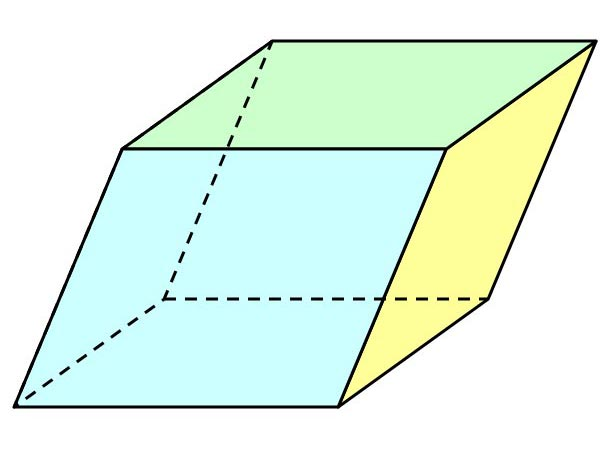
\includegraphics[width=3cm]{pp.jpg}}}
	\put(1.,0.25){$\r$}
	\put(0.5,0.6){$\mathbf{v}_{rel}$}
	\put(0.2,0.9){$\mathbf{a}$}
	\end{picture}}
	\item violated for planar relative orbits
	\end{itemize}
%\vspace*{0.3cm}\pause
\item How observable is a relative orbit? Goal: define a measure of observability.
\end{itemize}

\end{frame}


\begin{frame}
\frametitle{Measure of Observability}

\begin{itemize}
\item Main idea: the linearized dynamics of a relative orbit are unobservable, but the nonlinear properties of these systems may increase the observability by some amount that we wish to measure.
\item Approach: define an observability Gramian, which measures the sensitivity of the output with respect to the relative orbit initial condition over the estimation time period:
\begin{align}
\mathcal{W} (\x_0,t_0,t_f) = \int_{t_0}^{t_f} \parenth{\deriv{\y(\tau)}{\x_0}}^T\deriv{\y(\tau)}{\x_0}\,d\tau,\label{eqn:Wo_NL}
\end{align}
which is numerically calculated element-by-element as
\begin{align}
[\mathcal{W}]_{ij} = \frac{1}{4\epsilon^2}\sum_{k=0}^N (\y^{i+}_k-\y^{i-}_k)(\y^{j+}_k-\y^{j-}_k) \Delta t_k.
\end{align}
\item The smaller $\mathrm{cond}\braces{\mathcal{W}}$ is, the more the nonlinear system becomes observable.
\end{itemize}

\end{frame}


\section*{}
\subsection*{IV. Numerical Example}

\begin{frame}
\frametitle{Numerical Examples}

\begin{itemize}
\item Orbital Properties
	\begin{itemize}
	\item Chief: a circular orbit with an orbital radius of $7100\,\mathrm{km}$ such that $x_{chief,0}=[5020,\ 5020,\ 0,\ -1.812,\ 1.812,\ 7.041]^T$
	\item Deputy orbits are chosen at various locations, with relative orbits plotted:
	\end{itemize}	
\end{itemize}
\begin{figure}[h]
\centerline{
	\subfigure[Case 0C]{
		\includegraphics[width=0.19\textwidth]{OM_IOD_0C_traj.pdf}}
	\hfill
	\subfigure[Case $\mathbf{1}$]{
		\includegraphics[width=0.19\textwidth]{OM_IOD_1_traj.pdf}}
	\hfill
	\subfigure[Case 2A]{
		\includegraphics[width=0.19\textwidth]{OM_IOD_2A_traj.pdf}}
	\hfill
	\subfigure[Case 3A]{
		\includegraphics[width=0.19\textwidth]{OM_IOD_3A_traj.pdf}}
	\hfill
	\subfigure[Case 4C]{
		\includegraphics[width=0.19\textwidth]{OM_IOD_4C_traj.pdf}}
}
\caption{An example from each set of relative trajectories (solid red: HCW, dashed blue: two-body solution). Better tracking was shown with those trajectories that changed with time (not entirely cyclic) or varied far from the linearized solution.}
\label{fig:0CasesTraj}
\end{figure}

%\begin{figure}[h]
%\label{fig:CaseTraj}
%\centerline{
%	\subfigure[Case 1]{
%		\includegraphics[width=0.3\textwidth]{OM_IOD_1_traj.pdf}}
%}
%\caption{The trajectory of the Case 1 (solid red: HCW, dashed blue: two-body solution) shows that the linear and nonlinear solutions are very close, where both solutions are largely planar and cyclic.}
%\label{fig:1CasesTraj}
%\end{figure}
%
%
%\begin{figure}[h]
%\centerline{
%	\subfigure[Case 2A]{
%		\includegraphics[width=0.3\textwidth]{OM_IOD_2A_traj.pdf}}
%	\hfill
%	\subfigure[Case 2B]{
%		\includegraphics[width=0.3\textwidth]{OM_IOD_2B_traj.pdf}}
%	\hfill
%	\subfigure[Case 2C]{
%		\includegraphics[width=0.3\textwidth]{OM_IOD_2C_traj.pdf}}
%}
%\caption{The trajectories of the Cases 2A, 2B, and 2C (solid red: HCW, dashed blue: two-body solution) show differences between the linear and nonlinear solutions that vary about the $y$-axis, increasing the observabilities.}
%\label{fig:2CasesTraj}
%\end{figure}
%
%\begin{figure}[h]
%\centerline{
%	\subfigure[Case 3A]{
%		\includegraphics[width=0.3\textwidth]{OM_IOD_3A_traj.pdf}}
%	\hfill
%	\subfigure[Case 3B]{
%		\includegraphics[width=0.3\textwidth]{OM_IOD_3B_traj.pdf}}
%	\hfill
%	\subfigure[Case 3C]{
%		\includegraphics[width=0.3\textwidth]{OM_IOD_3C_traj.pdf}}
%}
%\caption{The trajectories of the Cases 3A, 3B, and 3C (solid red: HCW, dashed blue: two-body solution) exhibit large observabilities due to nonlinear solutions that move far away from the linearized solutions.}
%\label{fig:3CasesTraj}
%\end{figure}
%
%\begin{figure}[h]
%\centerline{
%	\subfigure[Case 4A]{
%		\includegraphics[width=0.3\textwidth]{OM_IOD_4A_traj.pdf}}
%	\hfill
%	\subfigure[Case 4B]{
%		\includegraphics[width=0.3\textwidth]{OM_IOD_4B_traj.pdf}}
%	\hfill
%	\subfigure[Case 4C]{
%		\includegraphics[width=0.3\textwidth]{OM_IOD_4C_traj.pdf}}
%}
%\caption{The trajectories of the Cases 4A, 4B, and 4C (solid red: HCW, dashed blue: two-body solution) experience the largest observabilities due to nonlinear solutions that move farther away from the linearized solutions than any of the trajectories from other cases considered in this paper.}
%\label{fig:4CasesTraj}
%\end{figure}

\end{frame}

\begin{frame}
\frametitle{Numerical Examples}
\framesubtitle{Observability Measure for the Various Cases}

\begin{itemize}
\item An initial orbit determination (IOD) approximation serves as the initial value for the Kalman filter.
\end{itemize}

\begin{center}
\resizebox{.5\columnwidth}{!}{
\begin{threeparttable}[h]
\caption{Case Observabilities and Initial Errors}
\begin{tabularx}{\textwidth}
{
>{$}c<{$}
*{1}{>{$}c<{$}} |
*{2}{>{$}c<{$}} |
*{2}{>{$}c<{$}}
}
\toprule
\multirow{2}{*}{Case} & \multirow{2}{*}{$\mathrm{cond}\braces{\mathcal{W}}$} & \multicolumn{2}{c}{\multirow{1}{*}{IOD1}} & \multicolumn{2}{c}{\multirow{1}{*}{IOD2}} \\
& &  e_{mag,0} & e_{dir,0} & e_{mag,0} & e_{dir,0} \\\midrule
0A & 10^{11.1486} & 0.0003 & 1.4901\times10^{-8} & 0.0012  & 2.1073\times10^{-8} \\
0B & 10^{10.9387} & 0.0233 & 0 & 0.0088 & 0 \\
0C & 10^{10.9851} & 0.0152 & 2.1073\times10^{-8} & 0.0139 & 1.4901\times10^{-8}  \\
\midrule
\mathbf{1} & 10^{16.6871} & 0.0001 & 0 & 0 & 0  \\
\midrule
2A & 10^{10.6492} & 0.0550 & 1.8150\times10^{-4} & 0.0238 & 1.8150\times10^{-4}  \\
2B & 10^{10.4163} & 0.9571 & 0.0734                     & 0.9571 & 0.0734  \\
2C & 10^{10.2155} & 0.0219 & 0.0044 & 0.0065 & 0.0044 \\
\midrule
3A & 10^{8.3490} & 0.0191 & 0.0031 & 0.1830 & 0.0031  \\
3B & 10^{8.5372} & 0.0612 & 0.0533 & 0.2315 & 0.0533  \\
3C & 10^{8.6586} & 6.8962 & 0.7348 & 5.4921 & 0.7348  \\
\midrule
4A & 10^{7.9062} & 8.7347 & 0.4587 & 0.1575 & 0.4587  \\
4B & 10^{7.9903} & 0.9276 & 0.1819 & 0.0621 & 0.1819  \\
4C & 10^{8.0645} & 0.1161 & 0.0554 & 0.0354 & 0.0554  \\
\bottomrule
\end{tabularx}
{\small
\begin{tablenotes}
    \item Note: $0$ indicates numbers small enough to be below Matlab numerical accuracy.
  \end{tablenotes}}
\label{tab:IODerr}
\end{threeparttable}
}
\end{center}
\vspace*{-0.1cm}
where $e_{mag,0}=\abs\left(1-{\frac{\norm{\r^+_0}}{\norm{\r_0}}}\right)$
and
$e_{dir,0}=\cos^{-1}\left(\frac{\r_0}{\norm{\r_0}}\cdot \frac{\r^+_0}{\norm{\r^+_0}}\right)$.

\end{frame}


\begin{frame}
\frametitle{Numerical Examples}
\framesubtitle{Kalman filter metrics with the two-body solution and $J_2$ effects}

\begin{center}
\begin{minipage}{0.45\columnwidth}
\resizebox{\columnwidth}{!}{
\begin{threeparttable}[h]
\caption{Error variables for EKF Considering Only Two-Body Problem Forces}
\begin{tabularx}{1.8\columnwidth}
{
>{$}c<{$}
*{1}{>{$}c<{$}} |
*{2}{>{$}c<{$}} |
*{2}{>{$}c<{$}}
}
\toprule
\multirow{2}{*}{Case} & \multirow{2}{*}{$\mathrm{cond}\braces{\mathcal{W}}$} & \multicolumn{2}{c}{IOD1} & \multicolumn{2}{c}{IOD2} \\
& & \bar e_{mag} & \bar e_{dir} & \bar e_{mag} & \bar e_{dir} \\\midrule
0A & 10^{11.1486} &  0.1918  &  0.0069  &  0.3140  &  0.0129 \\
0B & 10^{10.9387} &  0.7262  &  0.0505  &  0.1571  &  0.0086\\
0C & 10^{10.9851} &  0.0900  &  0.0061 &  0.1002  &  0.0154\\
\midrule
\mathbf{1} & 10^{16.6871} & \cellcolor{green} 4.059  & \cellcolor{green}  0.0109 & \cellcolor{green} 42.381 & \cellcolor{green}  0.0445 \\
\midrule
2A & 10^{10.6492} &  0.1978  &  0.0047  &  0.1638  &   0.0065   \\
2B & 10^{10.4163} & \cellcolor{green}  0.9853  & \cellcolor{green}  0.9307 & \cellcolor{green}  0.9278 & \cellcolor{green}   0.0114 \\
2C & 10^{10.2155} & 0.0563 &  0.0047 & 0.0536 &  0.0059 \\
\midrule
3A & 10^{8.3490} &  0.0516 & 0.0041   &  0.0643  &  0.0053 \\
3B & 10^{8.5372} &  0.0739  &  0.0035 &  0.1485 &  0.0071 \\
3C & 10^{8.6586} & \cellcolor{green}  2.063 & \cellcolor{green} 0.1614    & \cellcolor{green}  10.136  & \cellcolor{green}   0.9195 \\
\midrule
4A & 10^{7.9062} & \cellcolor{green}  6.359  & \cellcolor{green} 1.4235  &  12.0062   &  1.5310  \\
4B & 10^{7.9903} & \cellcolor{green}  0.2773  & \cellcolor{green}  0.0814   &  0.5244  &  0.2305 \\
4C & 10^{8.0645} &  2.0105 &  0.9144   &  0.0303 &  0.0036 \\
\bottomrule
\end{tabularx}
{\small
\begin{tablenotes}
    \item \hilight{Filter diverges}
  \end{tablenotes}}
\label{tab:ResultsTBP}
\end{threeparttable}
}
\end{minipage}
\begin{minipage}{0.45\columnwidth}
\resizebox{\columnwidth}{!}{
\begin{threeparttable}[h]
\caption{Error variables for EKF Considering Only Two-Body Problem Forces}
\begin{tabularx}{1.8\columnwidth}
{
>{$}c<{$}
*{1}{>{$}c<{$}} |
*{2}{>{$}c<{$}} |
*{2}{>{$}c<{$}}
}
\toprule
\multirow{2}{*}{Case} & \multirow{2}{*}{$\mathrm{cond}\braces{\mathcal{W}}$} & \multicolumn{2}{c}{IOD1} & \multicolumn{2}{c}{IOD2} \\
& & \bar e_{mag} & \bar e_{dir} & \bar e_{mag} & \bar e_{dir} \\\midrule
0A & 10^{11.1486} &  0.3766  &  0.0144  &  0.5145  &  0.0691 \\
0B & 10^{10.9387} &  0.5186  &  0.0810  &  0.3092  &  0.0804\\
0C & 10^{10.9851} &  0.2723  &  0.1362 &  0.1707 &  0.0614\\
\midrule
\mathbf{1} & 10^{16.6871} & \cellcolor{green} 4.078  & \cellcolor{green}  0.0109 & \cellcolor{green} 42.486 & \cellcolor{green}  0.0445 \\
\midrule
2A & 10^{10.6492} &  0.1592  &   0.0043  &  0.1348  &   0.0065   \\
2B & 10^{10.4163} & \cellcolor{green} 0.9843   & \cellcolor{green}  0.0114  & \cellcolor{green}  0.9278 & \cellcolor{green}   0.0113 \\
2C & 10^{10.2155} & 0.0258 &  0.0044 & 0.0360 &  0.0059 \\
\midrule
3A & 10^{8.3490} &  0.0486 & 0.0040   &  0.0603  &  0.0053 \\
3B & 10^{8.5372} &  0.0680  &  0.0033 &  0.1459 &  0.0070 \\
3C & 10^{8.6586} & \cellcolor{green}  2.0611 & \cellcolor{green}  0.1595   & \cellcolor{green}  10.567  & \cellcolor{green}   0.9011 \\
\midrule
4A & 10^{7.9062} & \cellcolor{green}  6.0706  & \cellcolor{green} 1.3182  &  11.8882   &  1.5319  \\
4B & 10^{7.9903} & \cellcolor{green}  0.2723  & \cellcolor{green}  0.0789   &  0.3155  &  0.1061 \\
4C & 10^{8.0645} &  2.3699 &  0.8486   &  0.0278 &  0.0034 \\
\bottomrule
\end{tabularx}
{\small
\begin{tablenotes}
    \item \hilight{Filter diverges}
  \end{tablenotes}}
\label{tab:ResultsTBP}
\end{threeparttable}
}
\end{minipage}
\end{center}
\resizebox{.9\columnwidth}{!}{
where $\bar e_{mag}=\left(\frac1N\sum_{k=1}^N\left\{1-{\frac{\norm{\r^+_k}}{\norm{\r_k}}}\right\}^2\right)^{\frac12}$ and $\bar e_{dir}=\left(\frac1N\sum_{k=1}^N
\left\{\cos^{-1}\left(\frac{\r_k}{\norm{\r_k}}\cdot \frac{\r^+_k}{\norm{\r^+_k}}\right)\right\}^{2}
\right)^{\frac12}$.
}


\end{frame}


%\begin{frame}
%\setcounter{subfigure}{0}
%\frametitle{Numerical Examples}
%\framesubtitle{Deputy inclination $i=20^\circ$}
%
%\begin{figure}
%\only<1>{
%\centerline{
%	\subfigure[Trajectory in the inertial frame]{
%		\includegraphics[width=0.5\columnwidth]{ISSFD14_i_20_OT_iner.pdf}}
%	\hspace*{0.05\textwidth}
%	\subfigure[Relative trajectory in the LVLH frame]{
%		\includegraphics[width=0.5\columnwidth]{ISSFD14_i_20_OT_lvlh.pdf}}
%}}
%\only<2>{
%\centerline{
%	\subfigure[Min. singular value of $\mathcal{O}$]{
%		\includegraphics[width=0.5\columnwidth]{ISSFD14_i_20_OT_sig.pdf}}
%	\hspace*{0.05\textwidth}
%	\subfigure[Condition number of $\mathcal{O}$]{
%		\includegraphics[width=0.5\columnwidth]{ISSFD14_i_20_OT_cond.pdf}}
%}}
%\only<3>{
%\centerline{
%	\subfigure[Estimation errors]{
%		\includegraphics[width=0.5\columnwidth]{PE_i_20_e.pdf}}
%	\hspace*{0.05\textwidth}
%	\subfigure[True $\|\x\|$ (red) and Estimated $\|\hat\x\|$ (blue)]{
%		\includegraphics[width=0.5\columnwidth]{PE_i_20_xx_norm.pdf}}
%}}
%\end{figure}
%\end{frame}


\begin{frame}
\setcounter{subfigure}{0}
\frametitle{Numerical Examples}
\framesubtitle{True and estimated solution with the Kalman fitler}

\begin{figure}[h]
\centerline{
	\subfigure[Case 0C, IOD1]{
		\includegraphics[width=0.2\textwidth]{Case0Cq1IOD1TBPnormX.pdf}}
	\hfill
	\subfigure[Case $\mathbf{1}$, IOD1]{
		\includegraphics[width=0.2\textwidth]{Case1q1IOD1TBPnormX.pdf}}
	\hfill
	\subfigure[Case 2A, IOD1]{
		\includegraphics[width=0.2\textwidth]{Case2Aq1IOD1TBPnormX.pdf}}
	\hfill
	\subfigure[Case 3A, IOD1]{
		\includegraphics[width=0.2\textwidth]{Case3Aq1IOD1TBPnormX.pdf}}
	\hfill
	\subfigure[Case 4C, IOD1]{
		\includegraphics[width=0.2\textwidth]{Case4Cq1IOD1TBPnormX.pdf}}
}
\centerline{
	\subfigure[Case 0C, IOD2]{
		\includegraphics[width=0.2\textwidth]{Case0Cq1IOD2TBPnormX.pdf}}
	\hfill
	\subfigure[Case $\mathbf{1}$, IOD2]{
		\includegraphics[width=0.2\textwidth]{Case1q1IOD2TBPnormX.pdf}}
	\hfill
	\subfigure[Case 2A, IOD2]{
		\includegraphics[width=0.2\textwidth]{Case2Aq1IOD2TBPnormX.pdf}}
	\hfill
	\subfigure[Case 3A, IOD2]{
		\includegraphics[width=0.2\textwidth]{Case3Aq1IOD2TBPnormX.pdf}}
	\hfill
	\subfigure[Case 4C, IOD2]{
		\includegraphics[width=0.2\textwidth]{Case4Cq1IOD2TBPnormX.pdf}}
}
\caption{The magnitudes of the relative states (solid red: true, blue dashed: estimated) are shown for various two-body propagated cases with close IOD estimates where the filter only diverges when the observability is low.}\label{fig:ExampesEachCase}
\end{figure}


\end{frame}


%\begin{frame}
%\setcounter{subfigure}{0}
%\frametitle{Numerical Examples}
%\framesubtitle{Deputy inclination $i=40^\circ$}
%
%\begin{figure}
%\only<1>{
%\centerline{
%	\subfigure[Trajectory in the inertial frame]{
%		\includegraphics[width=0.5\columnwidth]{ISSFD14_i_40_OT_iner.pdf}}
%	\hspace*{0.05\textwidth}
%	\subfigure[Relative trajectory in the LVLH frame]{
%		\includegraphics[width=0.5\columnwidth]{ISSFD14_i_40_OT_lvlh.pdf}}
%}}
%\only<2>{
%\centerline{
%	\subfigure[Min. singular value of $\mathcal{O}$]{
%		\includegraphics[width=0.5\columnwidth]{ISSFD14_i_40_OT_sig.pdf}}
%	\hspace*{0.05\textwidth}
%	\subfigure[Condition number of $\mathcal{O}$]{
%		\includegraphics[width=0.5\columnwidth]{ISSFD14_i_40_OT_cond.pdf}}
%}}
%\only<3>{
%\centerline{
%	\subfigure[Estimation errors]{
%		\includegraphics[width=0.5\columnwidth]{PE_i_40_e.pdf}}
%	\hspace*{0.05\textwidth}
%	\subfigure[True $\|\x\|$ (red) and Estimated $\|\hat\x\|$ (blue)]{
%		\includegraphics[width=0.5\columnwidth]{PE_i_40_xx_norm.pdf}}
%}}
%\end{figure}
%\end{frame}


\begin{frame}
\setcounter{subfigure}{0}
\frametitle{Numerical Examples}
\framesubtitle{Plotted $J_2$ Perturbation Effects}

%\begin{itemize}
%\item Results show $J_2$ perturbations have little effect.
%\end{itemize}

\begin{figure}[h]
\centerline{
	\subfigure[State magnitude with the two-body solution]{
		\includegraphics[width=0.2\textwidth]{Case3Bq1IOD1TBPnormX.pdf}}
\hspace*{0.07\textwidth}
	\subfigure[State magnitude with the $J_2$ solution]{
		\includegraphics[width=0.2\textwidth]{Case3Bq1IOD1HighFidelitynormX.pdf}}
}
\centerline{
	\subfigure[Uncertainty measure with the two-body solution]{
		\includegraphics[width=0.2\textwidth]{Case3Bq1IOD1TBPeigP.pdf}}
\hspace*{0.07\textwidth}
	\subfigure[Uncertainty measure with the $J_2$ solution]{
		\includegraphics[width=0.2\textwidth]{Case3Bq1IOD1eigP.pdf}}
}
\caption{The magnitudes and maximum eigenvalues of the state covariance matrices of the relative states (solid red: true, blue dashed: estimated) in Case 3B with IOD1 serve as an example where the $J_2$ propagated simulations give very close results to those of the two-body solution.
}\label{fig:TBPvsJ2}
\end{figure}

\end{frame}


\begin{frame}
\frametitle{Numerical Examples}
\framesubtitle{Summary}

\begin{itemize}
\item Success or failure of the Kalman filter using angles-only measurements for relative orbit estimation depends on 2 criteria:
\begin{enumerate}
\item If the condition number of $\mathcal{W}$ is smaller, then the observability of the nonlinear system is greater.
\item If the IOD or an initial estimate is far from the truth, then the Kalman filter may not converge on the true solution.
\end{enumerate}
\item The $J_2$ perturbations had an insignificant effect on the results of these simulations.
\end{itemize}

\end{frame}

\section*{}
\subsection*{V. Conclusions}

\begin{frame}
\frametitle{Conclusions}

\begin{itemize}
\item When linearized dynamics are considered for angles-only relative orbit estimation, the system is unobservable.
\item When certain criteria are met, the unobservable linearized systems become observable if the nonlinear properties of those systems are considered.
\item An observability measure is derived to quantify the degree to which relative orbits become observable.
\item A Kalman filter serves to show how cases with greater observability (shown by the proposed measure) are more likely to converge on the true solution provided an accurate IOD estimate.
\item Cases with greater observability tend to converge more accurately to the true solution.
\item When $J_2$ perturbations are included into the process model, the Kalman filter performs similarly.
\end{itemize}

\end{frame}
\end{document}






















